% -*- coding: utf-8 -*-
% !TEX encoding = UTF-8 Unicode
% !TEX root =  main.tex

\chapter{Aufbau der PMSM und Regelungskomponenten mit Simulink}
\label{cha:regelungpmsm}

Die Einführung in das Kapitel stellt dem Leser zunächst eine grundlegende Einführung in die Modellierungssoftware  Simulink$^\text{\textregistered}$ geben, welches als Toolbox in der Software MATLAB$^\text{\textregistered}$ implementiert ist.
Somit erhalten auch Leser ohne Erfahrungen mit dem Softwarepaket, die zum weiteren Verständnis der Arbeit benötigten Grundkenntnisse.
Der Vorteil bei der Nutzung von Matlab basiert zum einen darauf, dass die Software etablierter Quasistandard in der Industrie und an Hochschulen ist, und zum andern auf der Anwenderfreundlichkeit bei der Durchführung von Simulationsprojekten. \autocite[Vorwort]{scherf2010}
Dem versierten Anwender der Software sei geraten, diesen Abschnitt zu überspringen.


\section{Einführung in Simulink}\label{sec:simulink}

MATLAB/Simulink ist vom Softwarehersteller \glqq{The Mathworks}\grqq ~entwickelt worden. Zu den Einsatzgebieten der Software zählen hauptsächlich Modellierung und Simulation technischer und physikalischer Systeme. 
MATLAB ist dabei die Kernsoftware, welche sich mit vielen Toolboxen ergänzen lässt. 
Der Name MATLAB wurde dabei von "MATrix LABoratory" abgeleitet.
Vor der Simulation eines technischen Prozesses steht die Modellbildung, welche in den vorangegangenen Kapiteln durchgeführt wurde.
Dazu sind die nötigen physikalischen Gesetzmäßigkeiten zur Beschreibung der Maschine und Regelung genutzt worden.
Als Ergebnis der Modellbildung werden nun die Differentialgleichungen, Verknüpfungen und Zusammenhänge innerhalb von Simulink zu einem geschlossen Simulationsmodell verbunden. 
Der Aufbau von den Systemen findet in Simulink mit Hilfe von Blockbildern statt, welche mit Signalflusspfeilen zu einem Signalflussplan kombiniert werden. 
Entscheident für die Simulation von dynamischen Systemen ist die Lösung von mathematischen Zusammenhängen, insbesondere von Differentialgleichungen. 
Zur Einführung in die Software dient daher ein einfaches physikalisches Simulationsbeispiel: das Pendel.

\subsection{Simulationsbeispiel -- Das mathematische Pendel}

Zur Modellbildung und Simulation eines dynamischen Fadenpendels sei zunächst die folgende Abbildung \ref{fig:pendel} gegeben:

\begin{figure}[h]
	\centering
	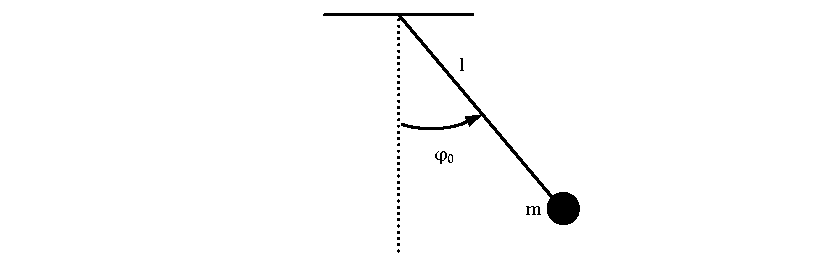
\includegraphics{/regelung/pendel.pdf}
	\label{fig:pendel}
	\caption{Fadenpendel}
\end{figure}

Er gelten folgende Momente:

Rückstellmoment
\begin{align}
		M_\i{R} = m \cdot g \cdot \si{sin}(\varphi) \label{rueckstellmoment} 
\end{align}
Beschleunigungsmoment
\begin{align}
	M_\i{B} = J \cdot \varphi = m \cdot l^{2} \cdot \ddot\varphi\label{beschleunigungsmoment} 
\end{align}
Reibungsmoment
\begin{align}
	M_\i{Reib} = d \cdot l^{2} \cdot \dot\varphi\label{reibungsmoment} 
\end{align}
Außerdem gilt:
\begin{align}
	\sum M = 0 \label{momentengleichgewicht} 
\end{align}

Die Bewegung des Pendels wird mit folgenden Werten simuliert:\\
\\
$ m = 2,3 ~\i{kg}\\ d = 0,2 ~\i{Nms}\\ l = 1,1 ~\i{m}\\ g = 9,81\tfrac{\i{m}}{\i{s^{2}}} \\ \varphi_\i{0} = 40^{\circ}$

Als nächster Schritt werden die physikalischen Systembeschreibungen in einer Gesamtformel zusammengefasst. 

\begin{align}
	\sum M = M_\i{R} + M_\i{B} + M_\i{Reib} = 0
	\label{momentengleichgewichtgesamt} 
\end{align}

\begin{align}
	\sum M = m \cdot g \cdot \si{sin}(\varphi) + J \cdot \varphi = m \cdot l^{2} \cdot \ddot\varphi + d \cdot l^{2} \cdot \dot\varphi = 0
	\label{momentengleichgewichtgesamt2} 
\end{align}

Wird nun die Differentialgleichung \ref{momentengleichgewichtgesamt2} nach der höchsten Ableitung $\ddot\varphi$ umgestellt, ergibt sich:

\begin{align}
	\ddot\varphi = -\dot\varphi \cdot \tfrac{\i{d}}{\i{m}} - \tfrac{\i{g}}{\i{l}} \cdot \si{sin}(\varphi)
	\label{diffgleichung} 
\end{align}

An dieser Stelle ist die Modellbildung abgeschlossen. Jetzt können die Werte in MATLAB/Simulink  verarbeitet werden.
Hier werden zuerst in der MATLAB-Umgebung Variablen mit den vorgegebenen Werten parametrisiert.

\begin{figure}[h]
	\centering
	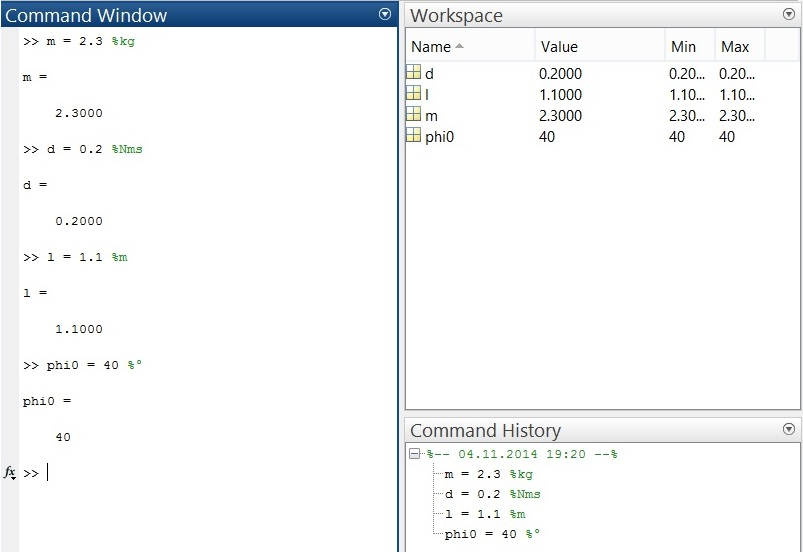
\includegraphics[width=\textwidth]{/regelung/matlab1.jpg}
	\label{fig:matlab1}
	\caption{Variablen in Matlab-Umgebung}
\end{figure}

Anschließend kann in der Simulink-Umgebung das Modell entsprechend \ref{momentengleichgewichtgesamt2} aufgebaut werden.

\begin{figure}[h]
	\centering
	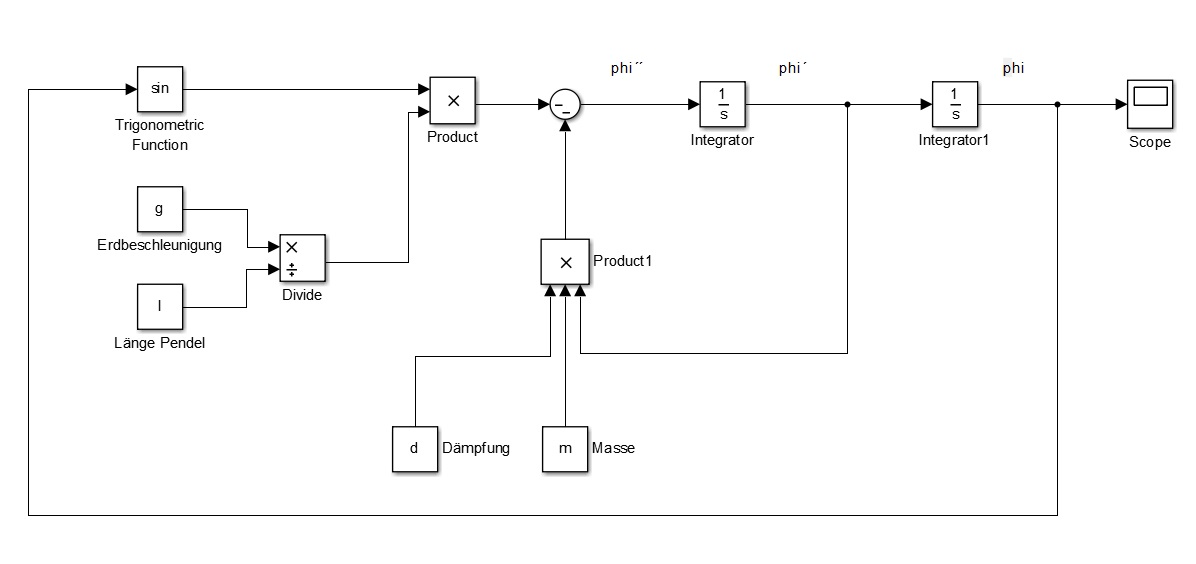
\includegraphics[width=\textwidth]{/regelung/matlab2.jpg}
	\label{fig:matlab2}
	\caption{fertiges Modell in Simulink}
\end{figure}

Herzstück des Simulationsmodells bilden zwei Integratoren.
Mit Hilfe dieser Blöcke lassen sich  $\dot{\varphi}$ und $\varphi$ erzeugen.
Die Simulink Bibliothek bietet eine Vielzahl von mathematischen Operatoren in Form von Blockbildern.
Mit Hilfe dieser Blöcke und der Signalflusspfeile lässt sich die Gleichung in das Simulationsmodell übertragen.
Ist das Modell aufgebaut, werden die Simulationsparameter ausgewählt. 
Simulink arbeitet numerisch, daher muss ein Integrationsverfahren zur Lösung der DGLs ausgewählt werden. Voreingestellt ist das Dormand-Prince-Verfahren mit variabler Schrittweite.
Diese Methode liefert in den meisten Anwendungen gute Ergebnisse. \autocite[S.~6]{scherf2010}
Zur Verifizierung der Simulationsergebnisse ist es für den Anwender unumgänglich, sich im Vorfeld Gedanken zum erwartenden Ergebnis zu machen.
Im vorliegenden Beispiel sollte der Winkel $\varphi$ eine gedämpfte Schwingung in Abhängigkeit von der Zeit erzeugen.
Das Ergebnis der Simulation erhält der Anwender beim Anwählen des Blockbildes \glqq{Scope}\grqq.
Hier zeigt sich nach durchgeführter Simulation folgendes Ergebnis:

\begin{figure}[h]
	\centering
	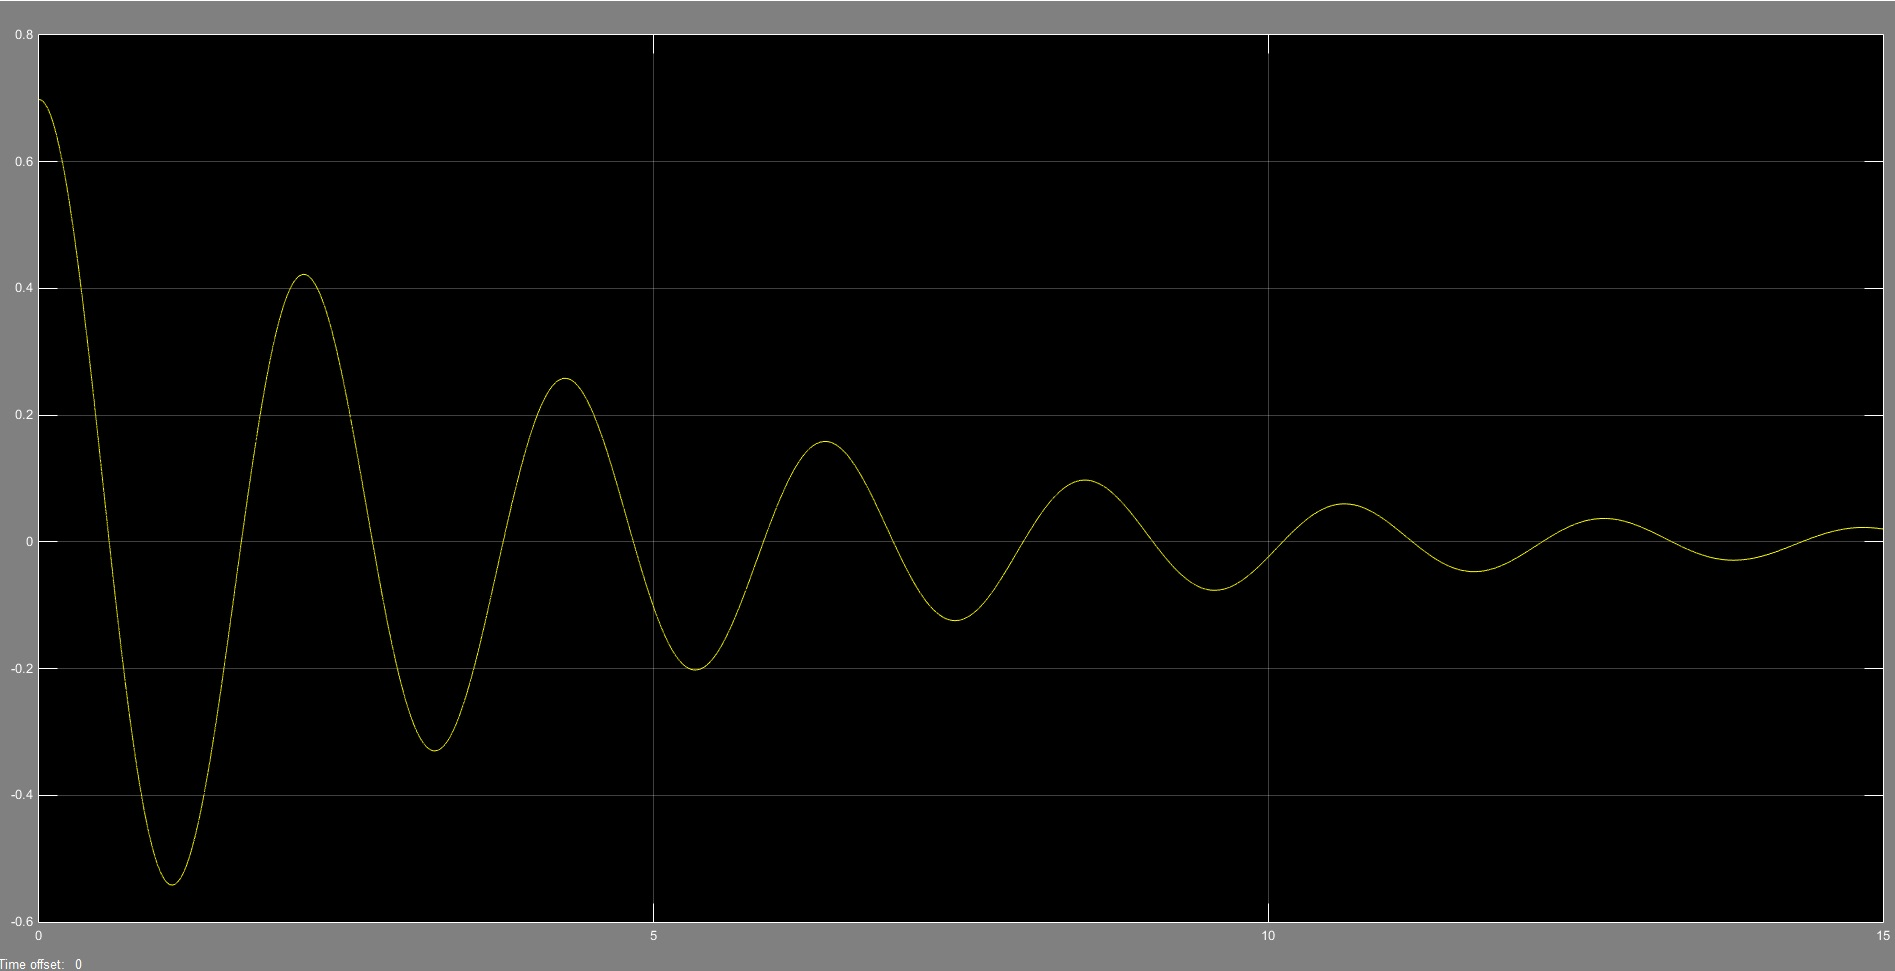
\includegraphics[width=\textwidth]{/regelung/matlab3.jpg}
	\label{fig:matlab3}
	\caption{ Winkel $\varphi$ des Pendels über die Simulationszeit t=15s}
\end{figure}


Wie erwartet, wird eine deutlich gedämpfte Schwingung des simulierten Pendels erkennbar.

\section{Simulationsblöcke}\label{sec:math-model-pmsm}

Dieses Kapitel dient zur Beschreibung der Bauteile und Komponenten, die für einen späteren Aufbau eines gesamten Regelungssystems der PMSM nötig sind.
Zunächst wird das erstellte Gesamtsystem in Abbildung \ref{fig:signalflussplan} dargestellt:

\begin{figure}[h]
	\centering
	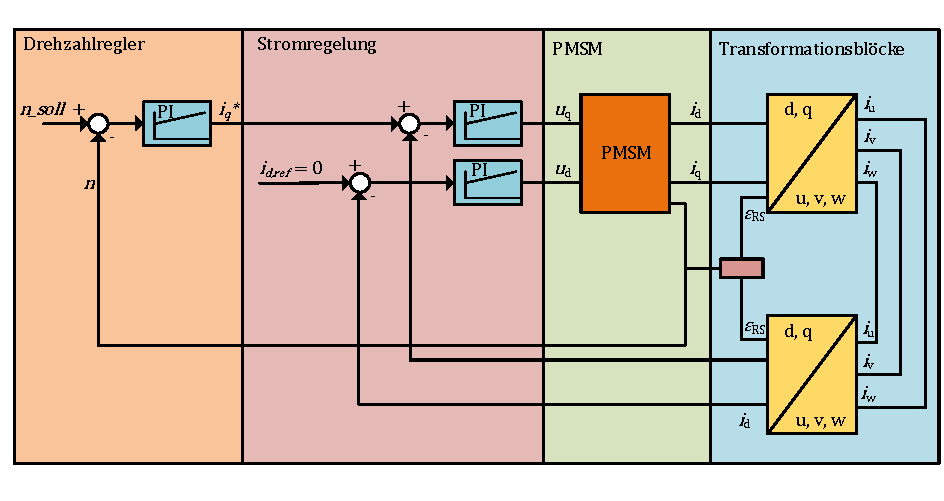
\includegraphics[width=\textwidth]{signalflussplan.pdf}
	\label{fig:signalflussplan}
	\caption{Signalflussplan}
\end{figure}

Hier sind die Simulinkblöcke der Transformationen, das Modell der PMSM sowie Regelungskomponenten erkennbar.
Im Folgenden werden diese erläutern und deren Funktionen dargestellt.

\subsection{Transformationsblöcke}

Der Aufbau der Koordinatentransformationen leitet aus Abschnitt \ref{sec:clark} ab. 
Hierbei basiert der Block der $\alpha$-$\beta$-Transformation aus den Zusammenhängen von (\ref{clarkevektor}) und (\ref{clarkematrix}), während die Rücktransformation, also die inverse $\alpha$-$\beta$-Transformation mit Hilfe von (\ref{inverseclarkevektornulleinfach}) und (\ref{inverseclarkematrixnulleinfach}) erstellt ist.
Weiterhin orientieren sich die Umsetzungen in Simulink an den Blockschaltbildern aus \ref{fig:blockbildclarkeparkkomplett} und \ref{fig:blockbildinverseclarkeparkkomplett}.

Die folgende Abbildung \ref{fig:uvw_to_ab} zeigt den Blockaufbau der Clarke Transformation in Simulink:

\begin{figure}[h]
	\centering
	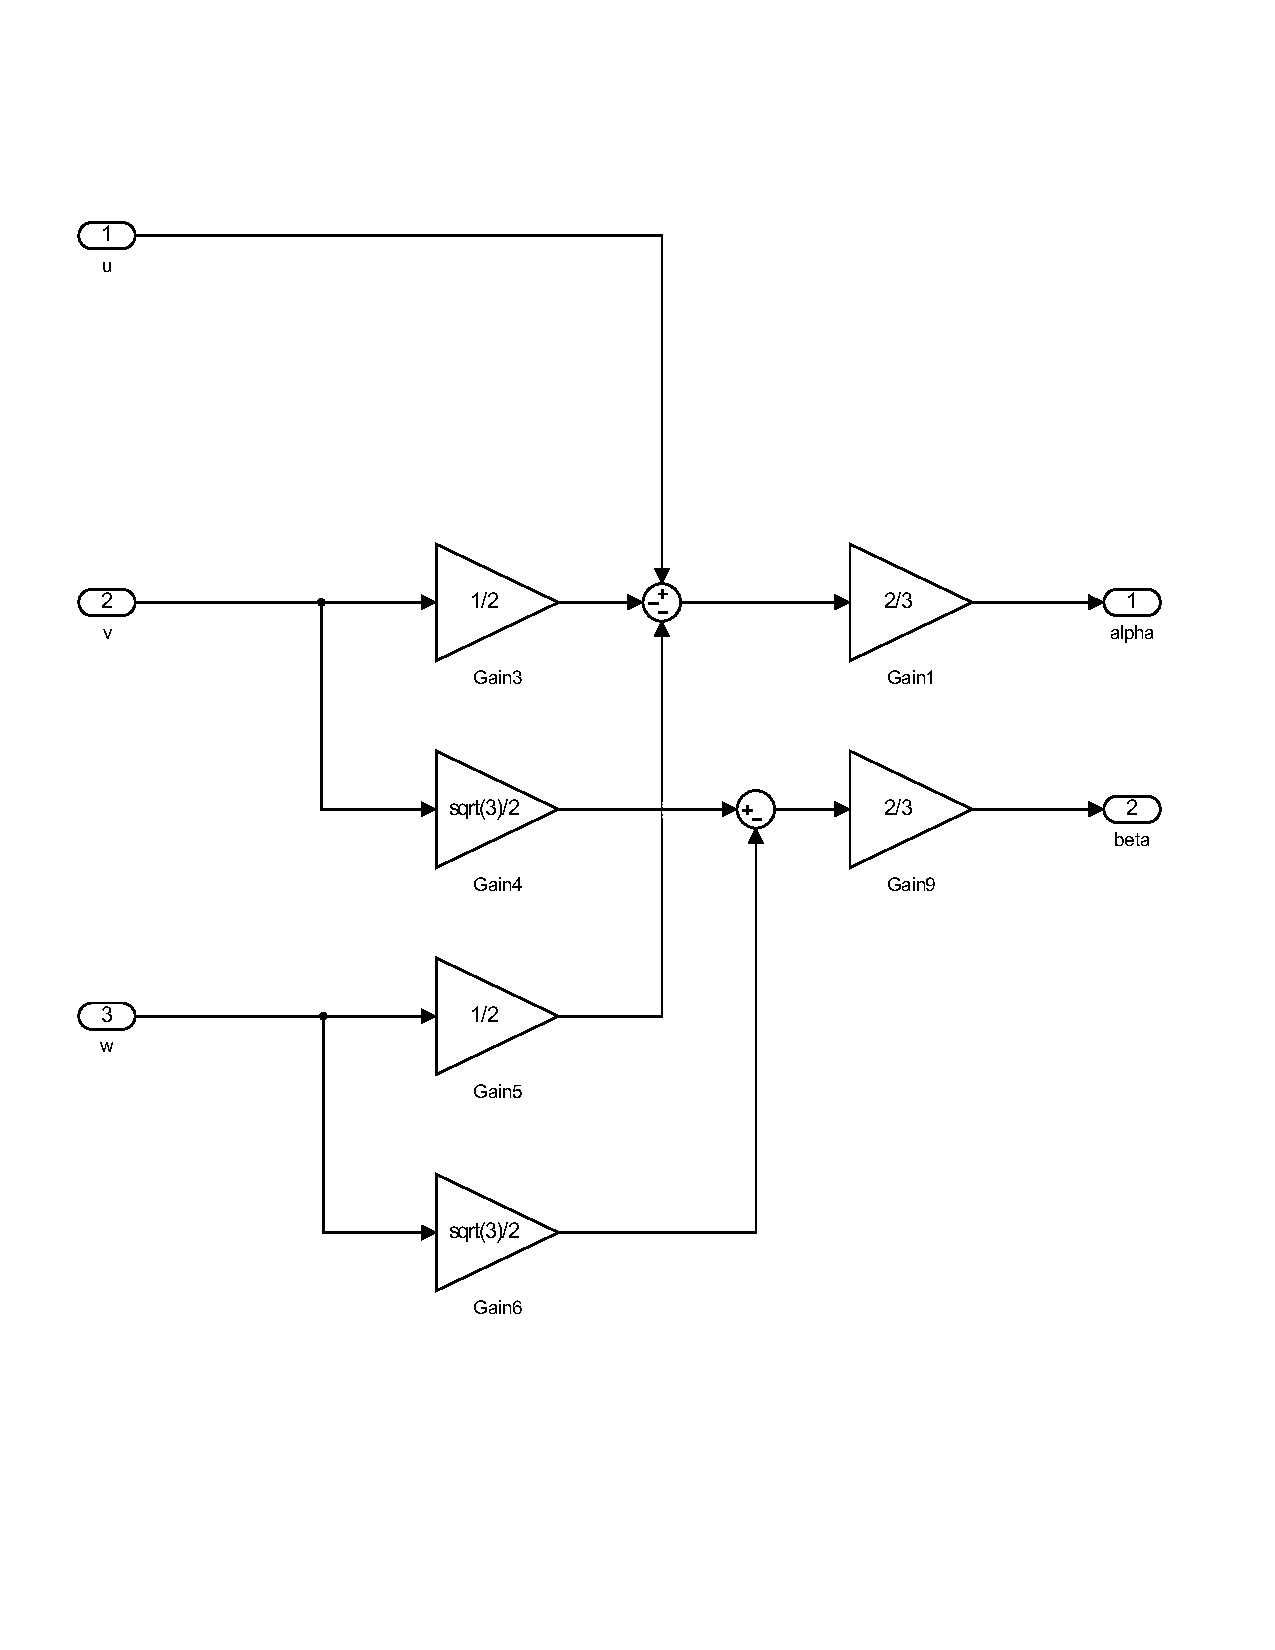
\includegraphics[width=\textwidth]{/simulink/uvw_to_ab.pdf}
	\label{fig:uvw_to_ab}
	\caption{Aufbau Clarke Transformation}
\end{figure}

In Abbildung \ref{fig:uvw_to_ab} wird der Aufbau der inversen Clarke Transformation gezeigt:

\begin{figure}[h]
	\centering
	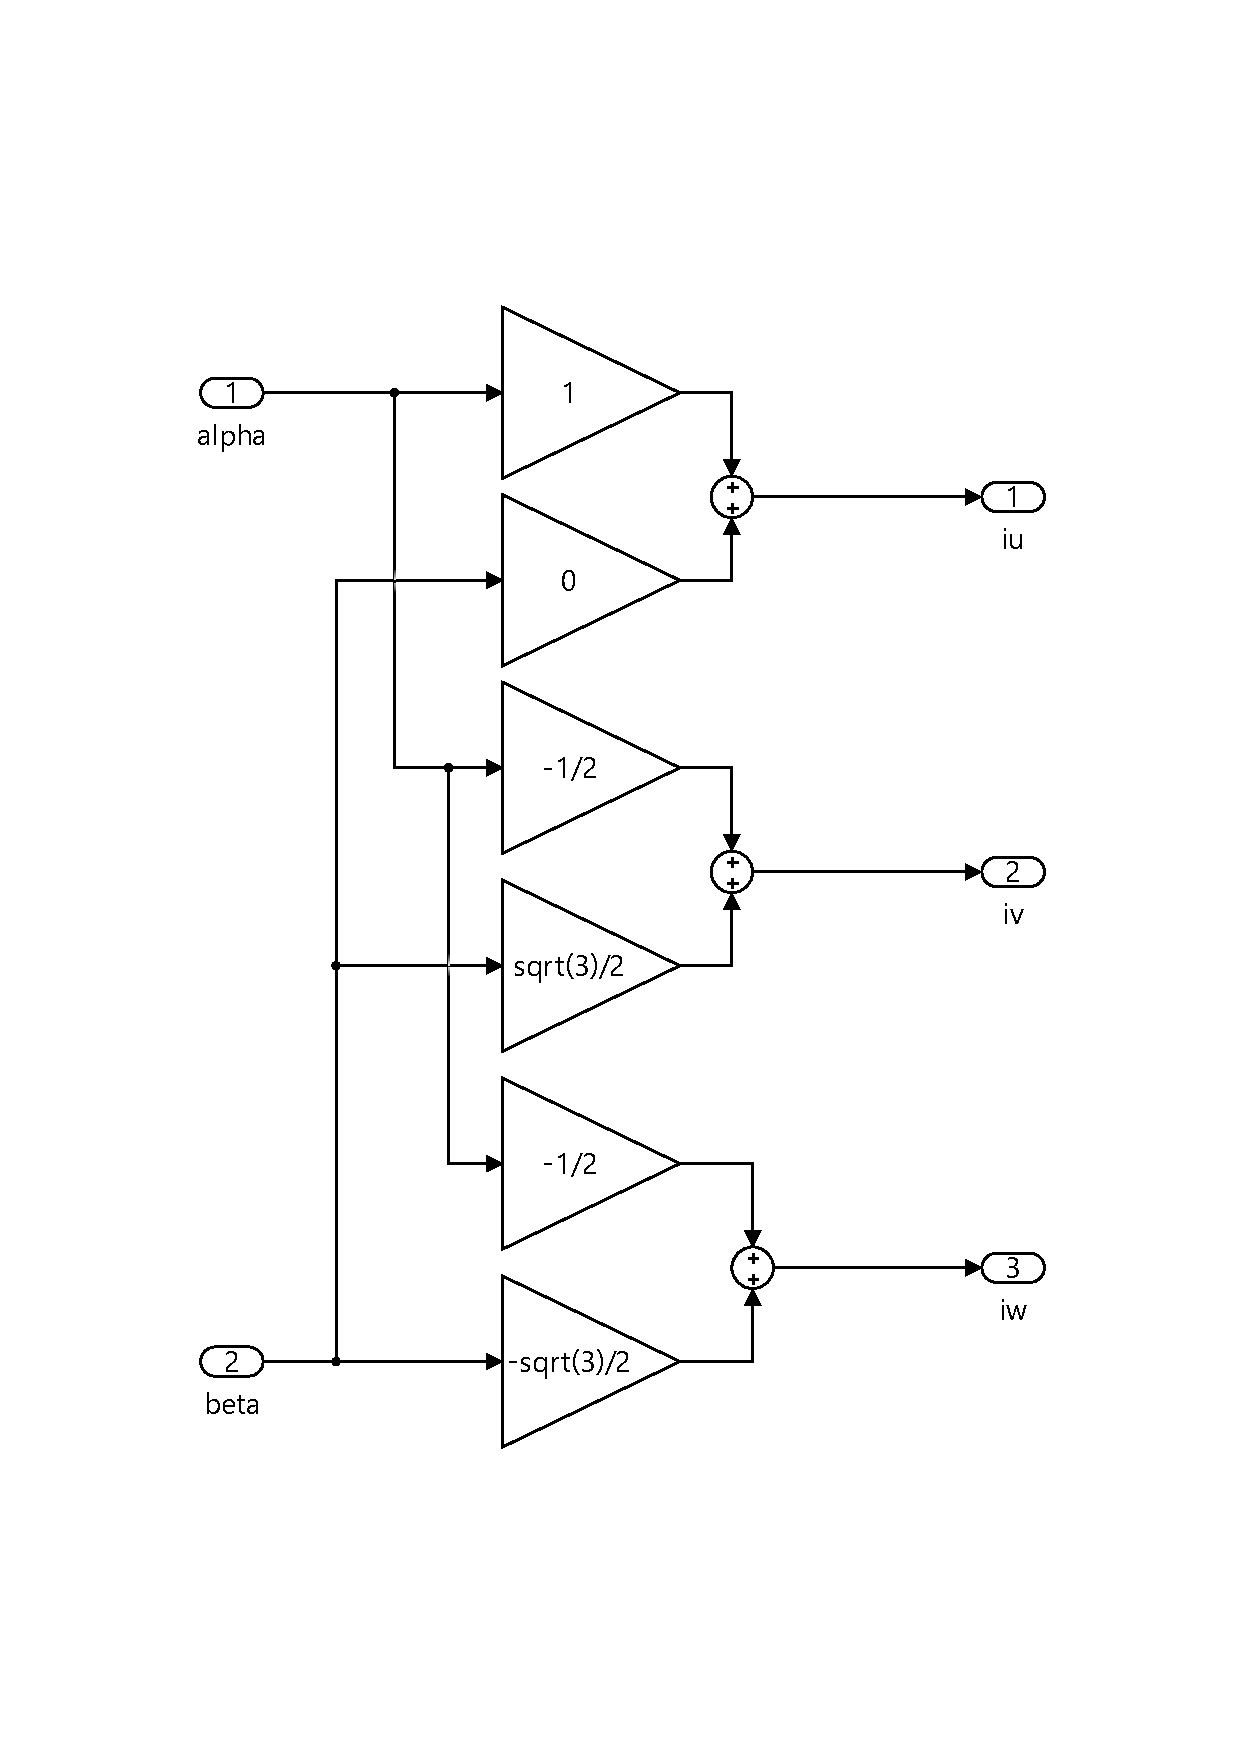
\includegraphics[width=\textwidth]{/simulink/ab_to_uvw.pdf}
	\label{fig:ab_to_uvw}
	\caption{Aufbau Inverse Clarke Transformation}
\end{figure}

Um die Koordinatentransformation zu vervollständigen ist die d-q-, oder Park Transformation, von entscheidender Bedeutung.
Der Block für die d-q-Transformation setzt wird mit dem Zusammenhang \ref{parkvektor} und der Matrix \ref{parkmatrix} erstellt. 
Die inverse d-q-Transformation ist mit Hilfe der Matritzen \ref{parkvektorinvers} sowie \ref{parkmatrixinvers} aufgebaut.

Die nachstehende Grafik \ref{fig:ab_to_dq} stellt die Park Transformation in Simulink dar:

\begin{figure}[h]
	\centering
	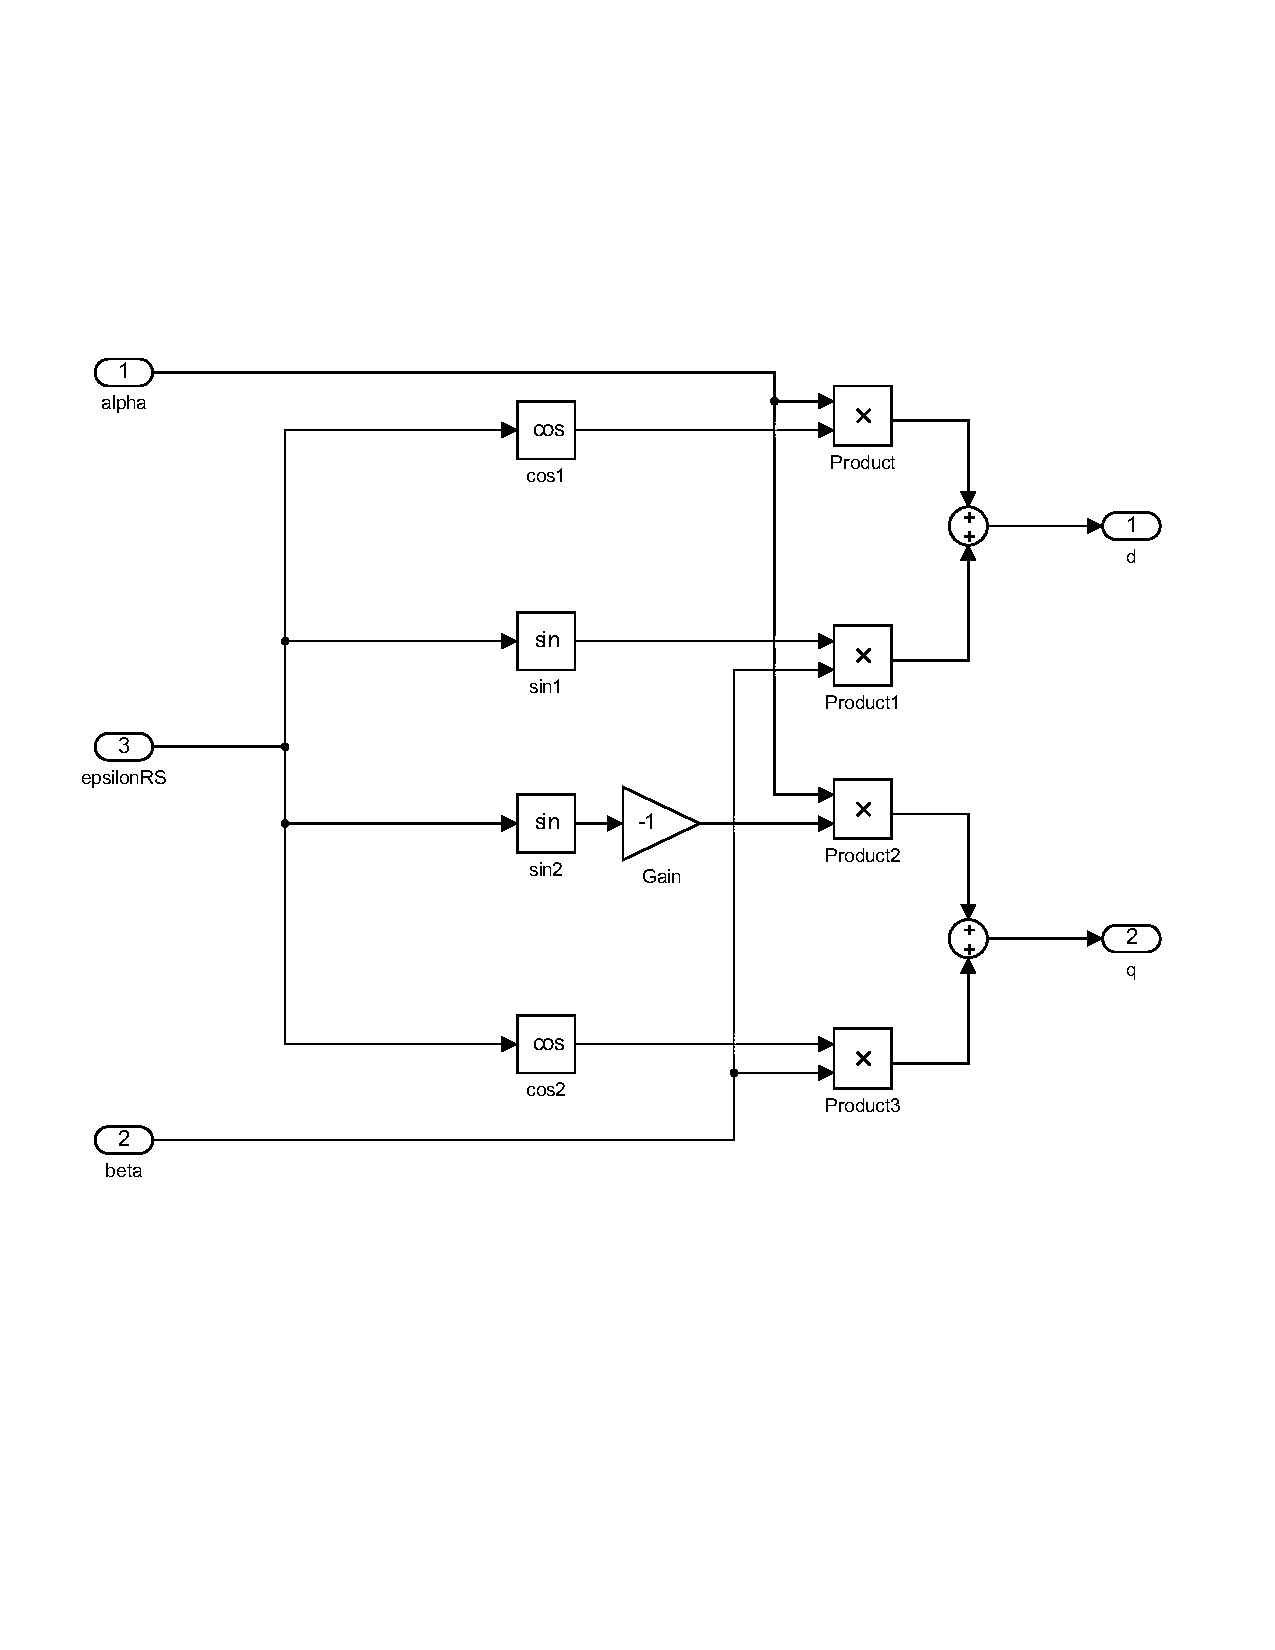
\includegraphics[width=\textwidth]{/simulink/ab_to_dq.pdf}
	\label{fig:ab_to_dq}
	\caption{Aufbau Park Transformation}
\end{figure}

In Abbildung \ref{fig:dq_to_ab} ist der Aufbau der inversen Park Transformation dargestellt:

\begin{figure}[h]
	\centering
	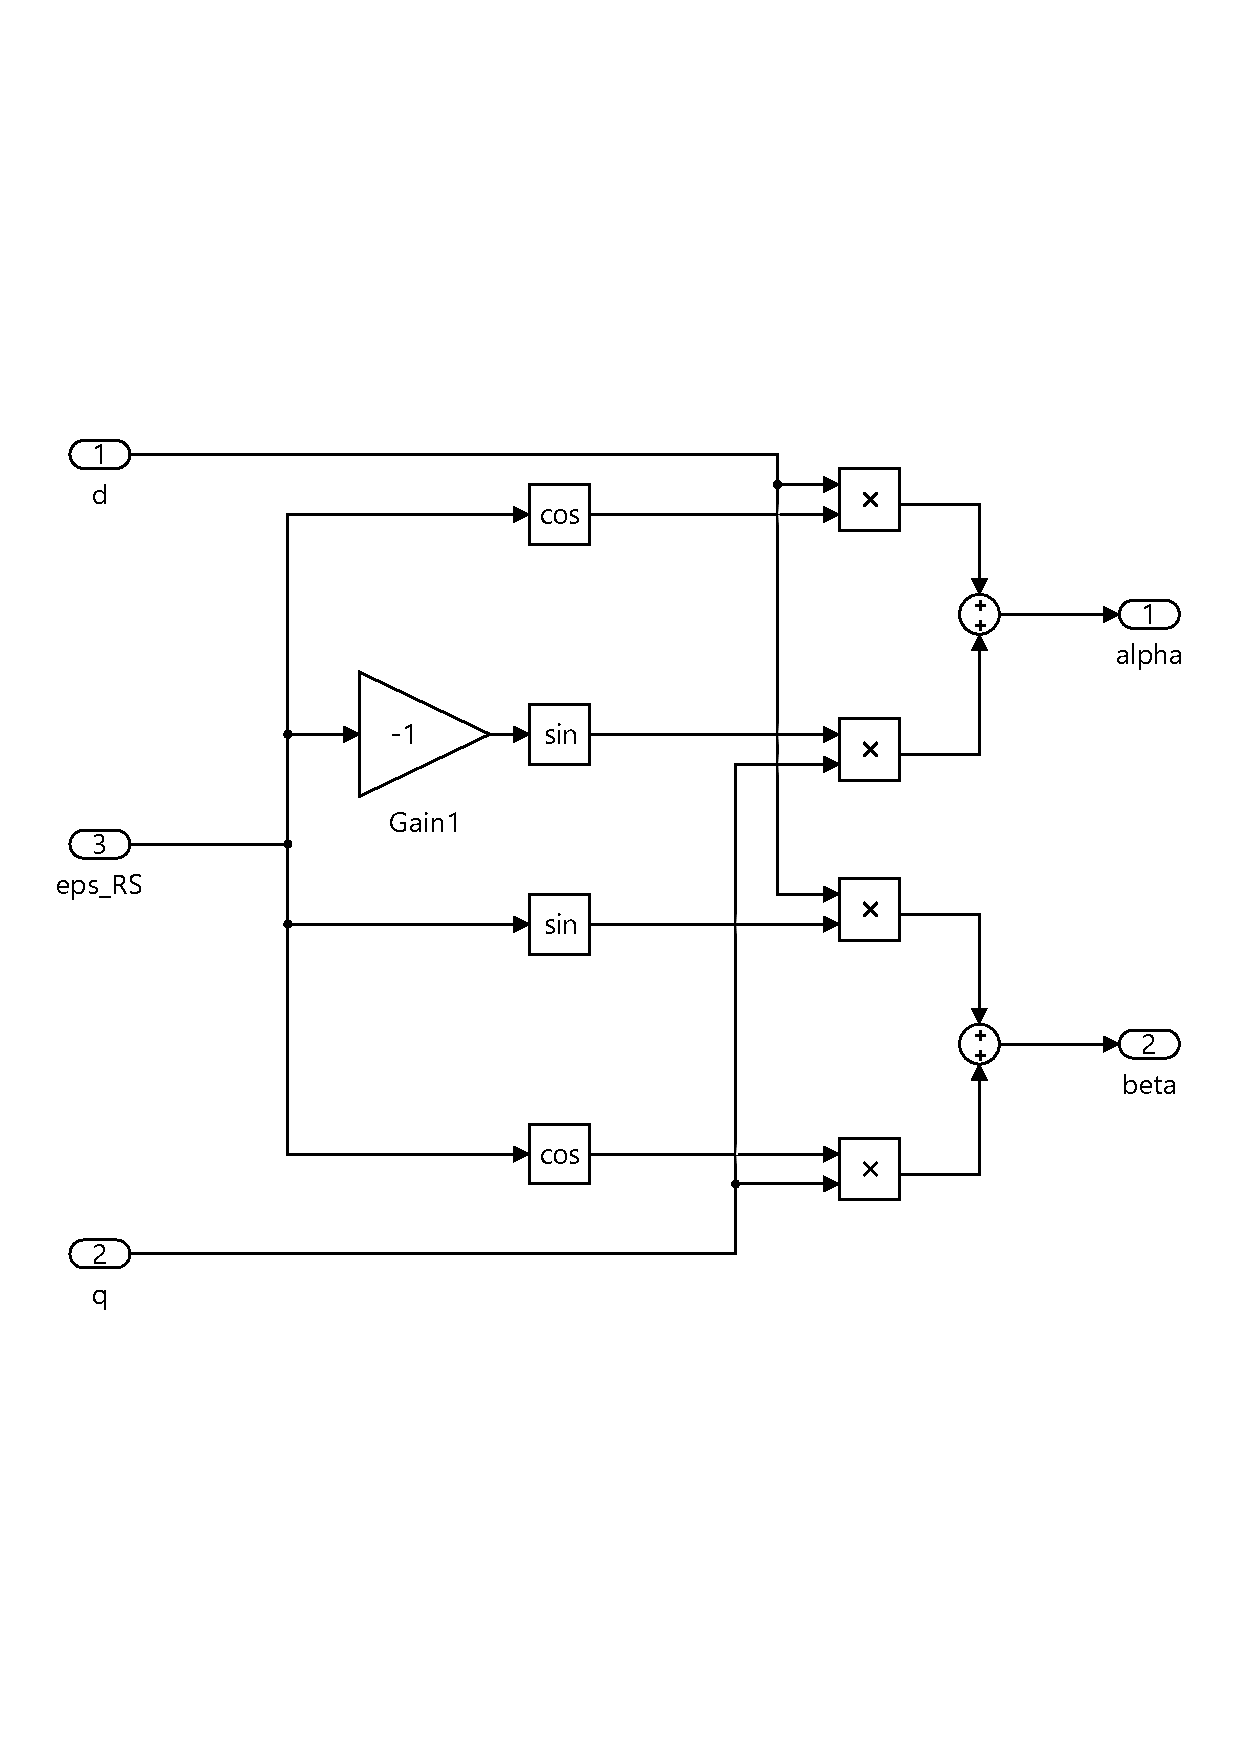
\includegraphics[width=\textwidth]{/simulink/dq_to_ab.pdf}
	\label{fig:dq_to_ab}
	\caption{Aufbau Inverse Park Transformation}
\end{figure}

An dieser Stelle ist es aus übersichtlichkeitsgründen sinnvoll, die Transformationsblöcke als Subsystem zusammenzufassen.
Es ergibt sich für die Clarke-Park Transformation somit ein Block mit drei Eingängen für die drei Wechselgrößen und einem Eingange für $\varepsilon_\i{RS}$, sowie zwei Ausgängen für d- und q-Komponente.

\begin{figure}[h]
	\centering
	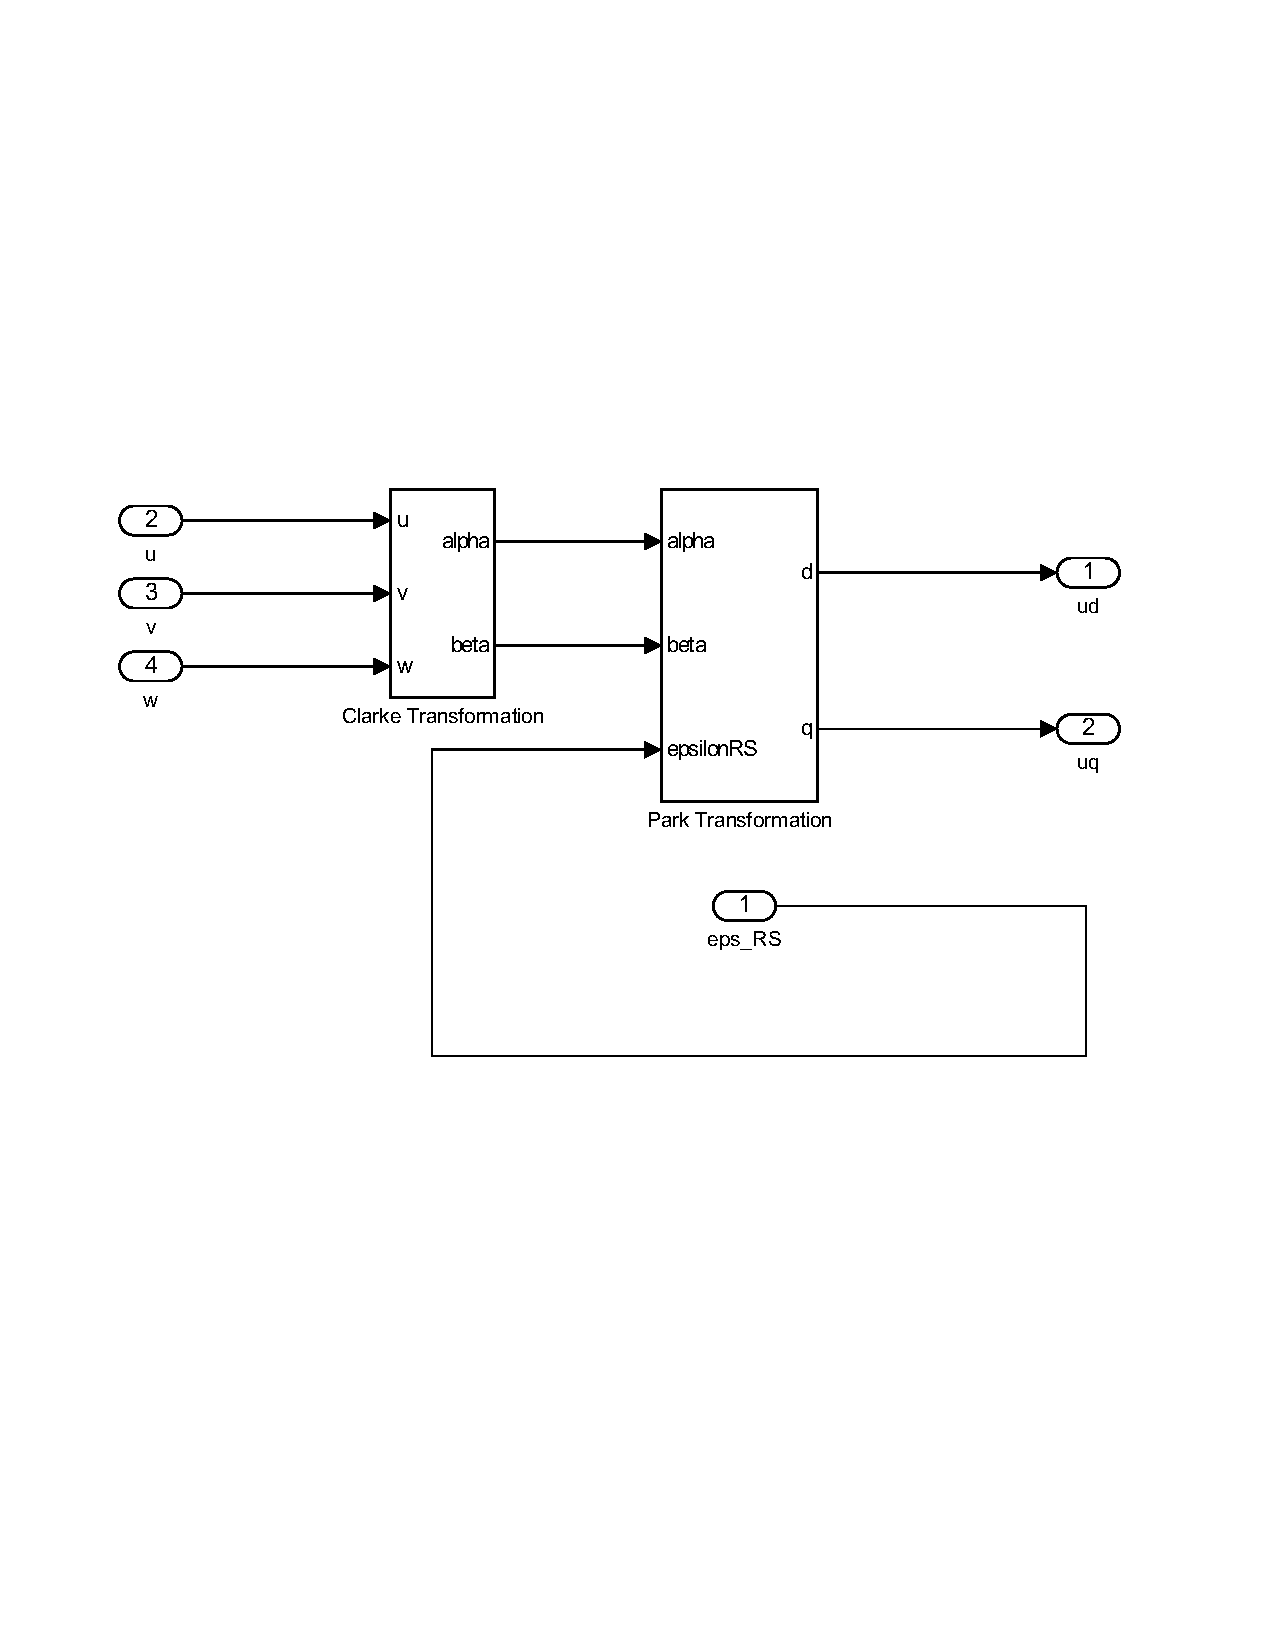
\includegraphics[width=\textwidth]{/simulink/uvw_to_dq.pdf}
	\label{fig:uvw_to_dq}
	\caption{Aufbau Clarke-Park Transformation}
\end{figure}

Ebendieses wird auch für die Rücktransformation gemacht. 
Hier ergibt sich ein Subsystem mit drei Eingängen. 
Zwei für d- und q-Größe sowie ebenfalls ein Eingang für $\varepsilon_\i{RS}$.
Es ergeben sich drei Ausgänge für das rückgeführte Dreiphasensystem.

\begin{figure}[h]
	\centering
	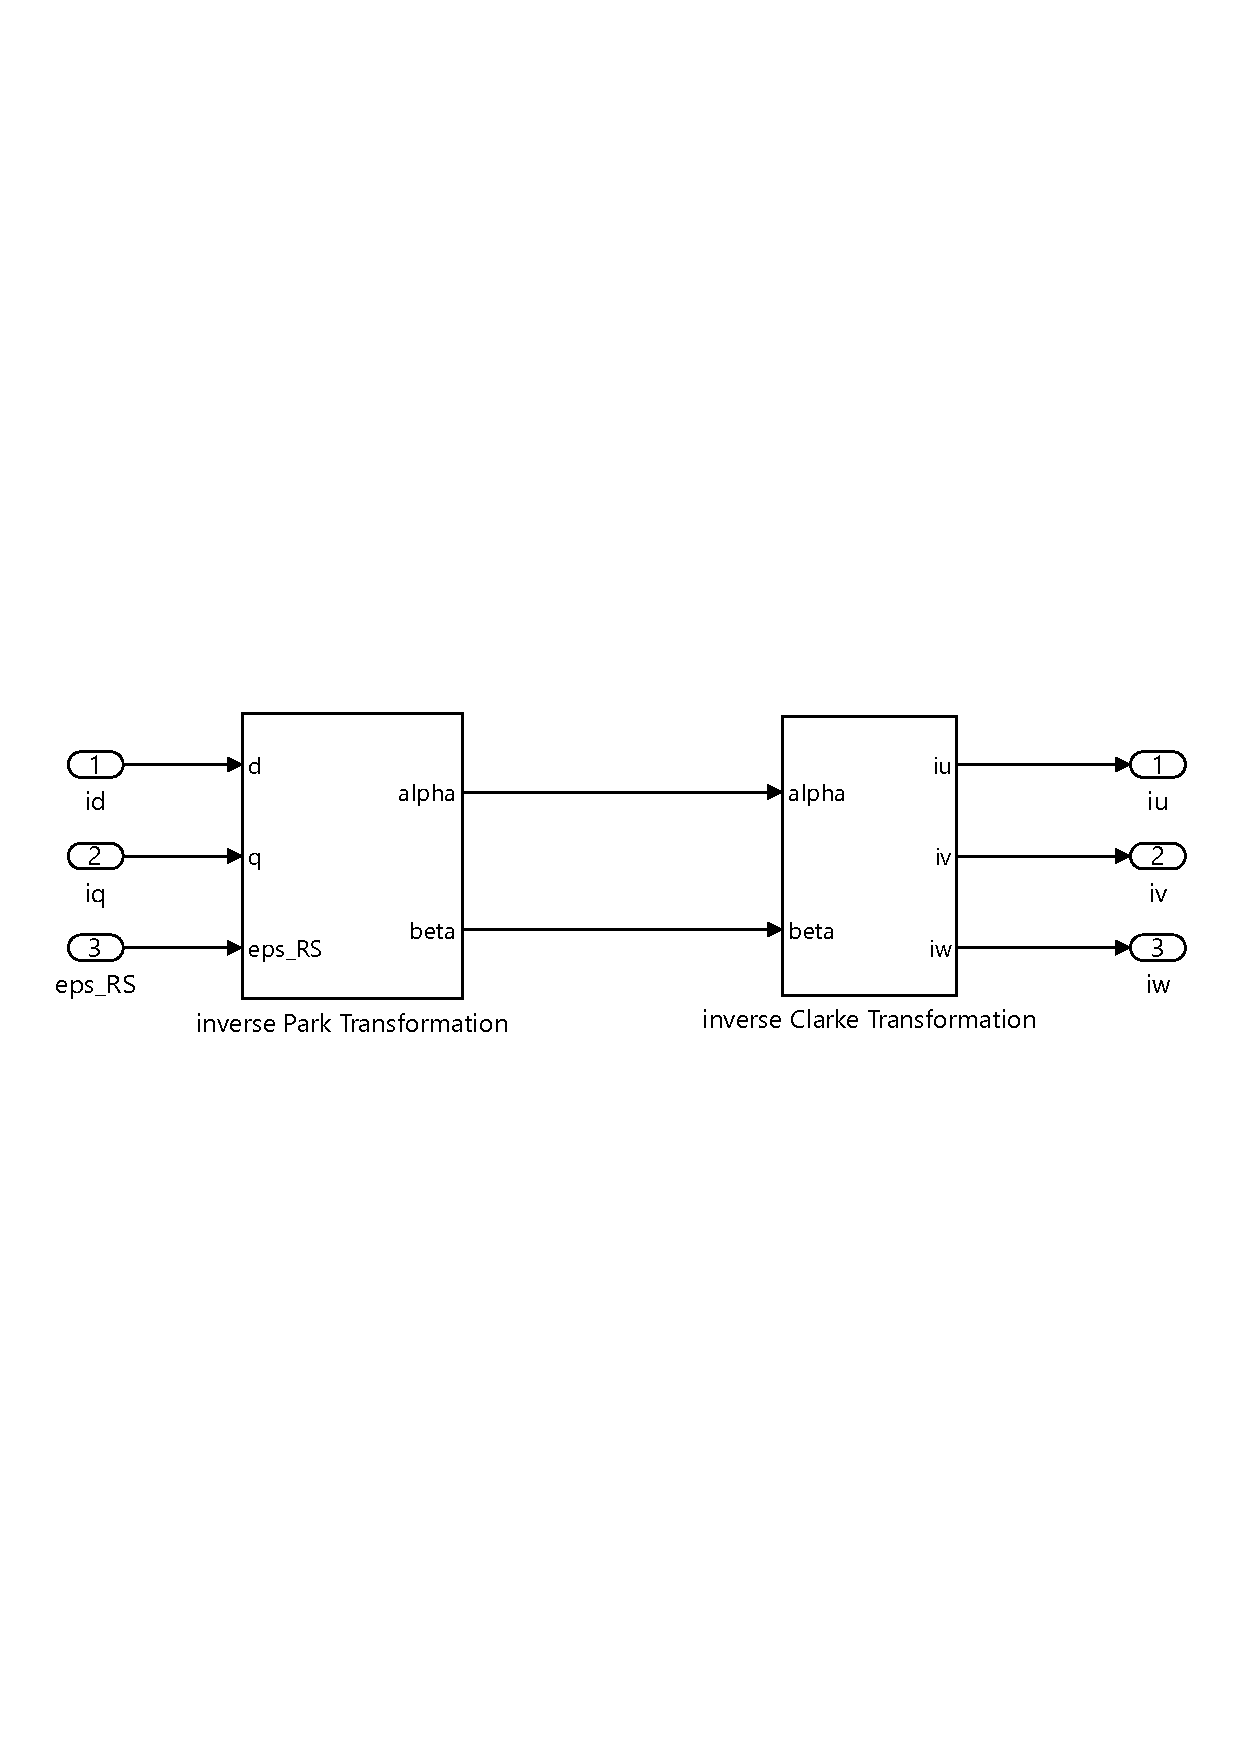
\includegraphics[width=\textwidth]{/simulink/dq_to_uvw.pdf}
	\label{fig:dq_to_uvw}
	\caption{Aufbau inverse Clarke-Park Transformation}
\end{figure}


\subsection{Modell der PMSM}

Als Grundlage für die Betrachtung der PMSM gilt der Abschnitt \ref{sec:synchron-dq}.
Die grundlegenden Gleichung dazu sind (\ref{eqn:ud-lin-gleichung}), (\ref{eqn:uq-lin-gleichung}) und (\ref{eqn:mi-lin-gleichung}).
Aus den Gleichungen ergibt sich dann im Simulink das Modell.
Das Modell wird in zwei Systeme unterteilt:

\begin{itemize}
	\item mechanical system
	\item electrical system
\end{itemize}

Bei dem \enquote{mechanical system} wird die Differentialgleichung der elektrischen Winkelgeschwindigkeit beschrieben.
Das \enquote{electrical system} beschreibt hingegen die Differentialgleichungen der Ströme und somit die elektrischen Parameter der PMSM.
Die Überführung der Maschinengleichungen erfolgt dabei dem gleichen Prinzip wie in Abschnitt \ref{sec:simulink}.
Zunächst wird auf das \enquote{electrical system} eingegangen, welches in Abbildung \ref{fig:electrical-system} dargestellt ist.

\begin{figure}[h]
	\centering
	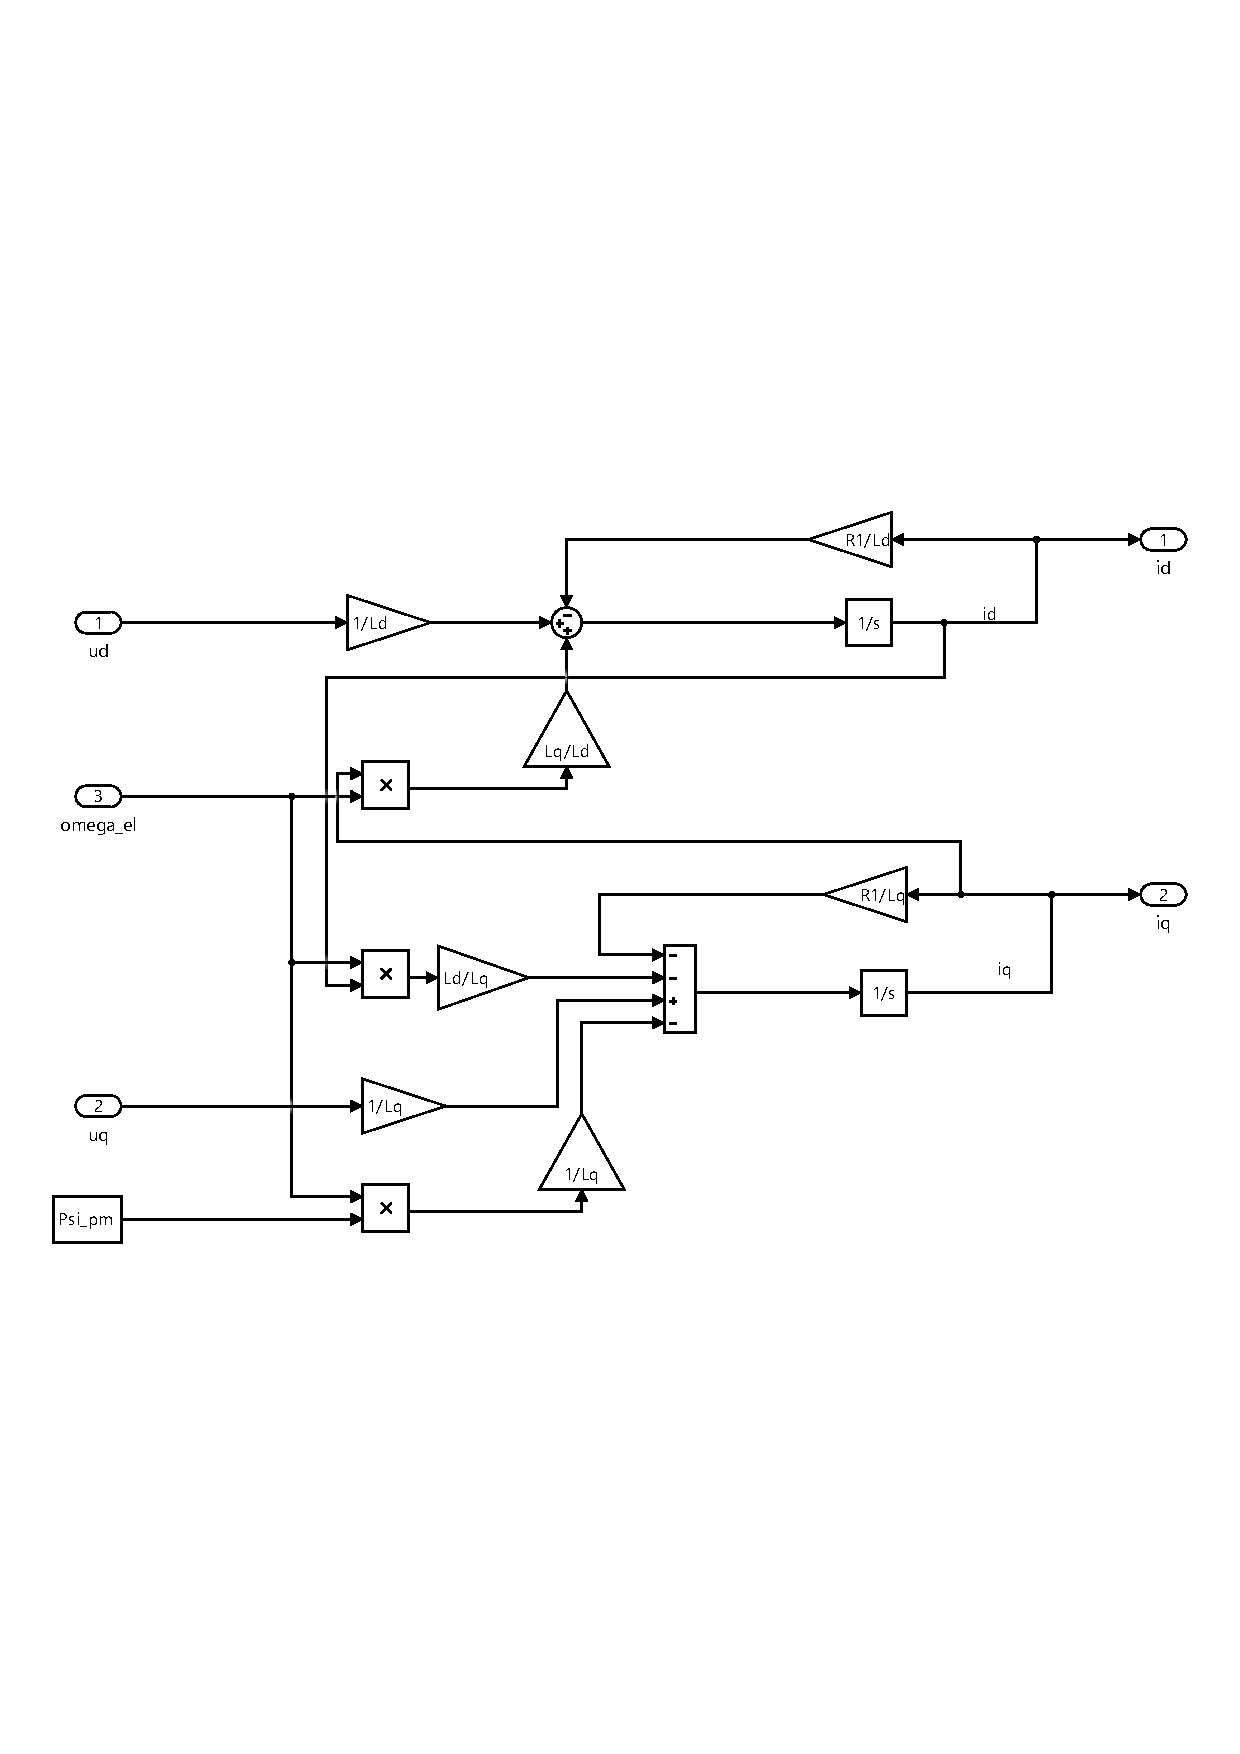
\includegraphics[width=\textwidth]{/simulink/electrical-system.pdf}
	\label{fig:electrical-system}
	\caption{Aufbau Subsystem \enquote{electrical system}}
\end{figure}

Das Subsystem ist mit den linearisierten Maschinengleichungen (\ref{eqn:ud-lin-gleichung}) und (\ref{eqn:uq-lin-gleichung}) aufgebaut. 
Aus den zugeführten Spannungen $u_\x{d}$ und $u_\x{d}$, sowie $\omega_\x{el}$ werden die Ströme $i_\x{d}$ und $i_\x{q}$ generiert.

Das \enquote{mechanical system} resultiert aus der Differentialgleichung des inneren Drehmomentes (\ref{eqn:mi-lin-gleichung}).

\begin{figure}[h]
	\centering
	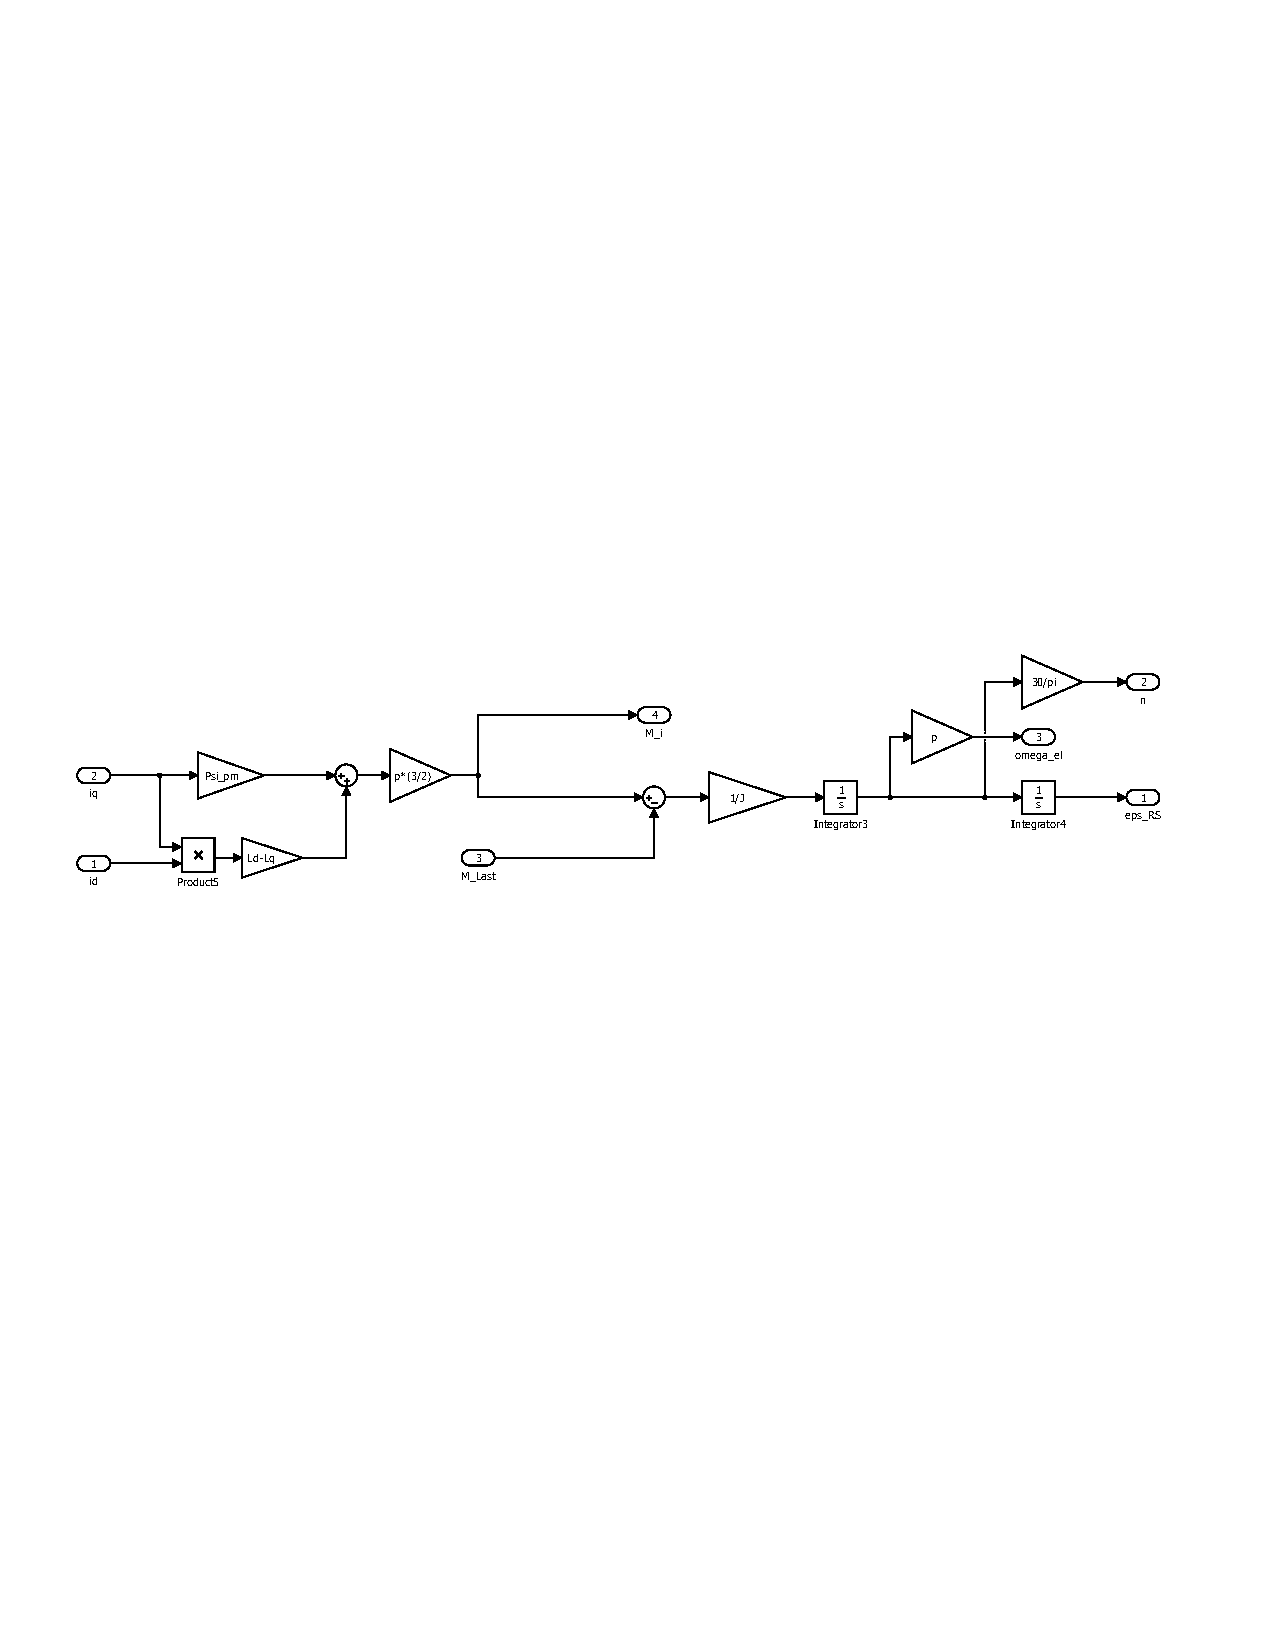
\includegraphics[width=\textwidth]{/simulink/mechanical-system.pdf}
	\label{fig:mechanical-system}
	\caption{Aufbau Subsystem \enquote{mechanical-system}}
\end{figure}

Im Subsystem, welches in Abbildung \ref{fig:mechanical-system} erkennbar ist, werden mit der d- und q-Komponente des Stromes aus dem \enquote{electrical system} das innere Drehmoment $M_\x{i}$, die Drehzahl, der elektrische Winkel $\omega_\x{el}$ sowie der Drehwinkel $\varepsilon_\i{RS}$.
Jetzt müssen die Subsysteme miteinander verknüpft werden.
So entsteht das Simulationsmodell der PMSM, welches im Gesamten in Abbildung \ref{fig:pmsm} dargestellt ist.

\begin{figure}[h]
	\centering
	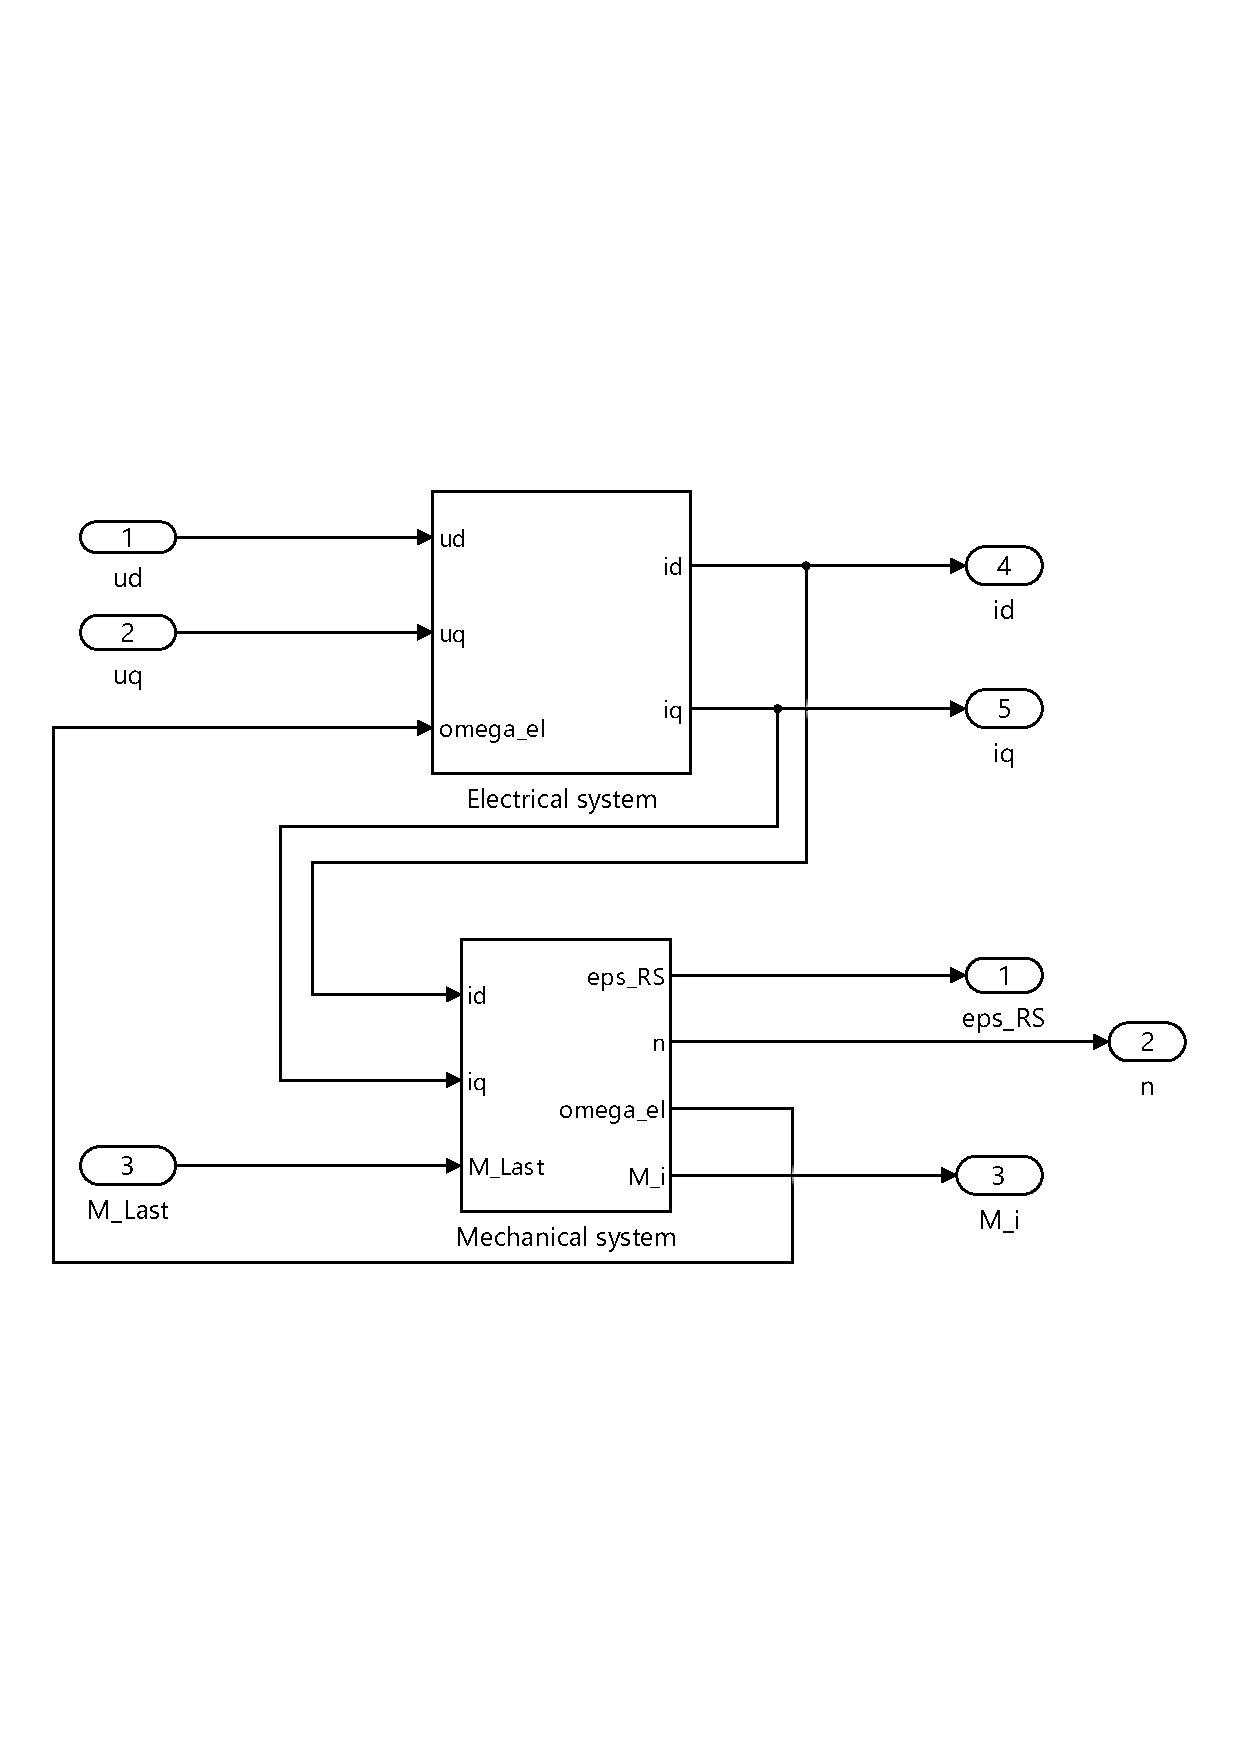
\includegraphics[width=\textwidth]{/simulink/pmsm.pdf}
	\label{fig:pmsm}
	\caption{Aufbau Subsystem der PMSM}
\end{figure}

\subsection{Regelblöcke}

Wie im Signalflussplan \ref{fig:signalflussplan} erkennbar, ist zum einen ein Drehzahlregler und zum anderen eine Stromregelung im Modell enthalten. 
Diese dienen dazu, um den Strom entsprechend der Solldrehzahl einzustellen.
Hierzu wurden einfache PI-Regler verwendet.
Die nachstehende Abbildung \ref{fig:drehzahl} zeigt den Aufbau Drehzahlregelung:

\begin{figure}[h]
	\centering
	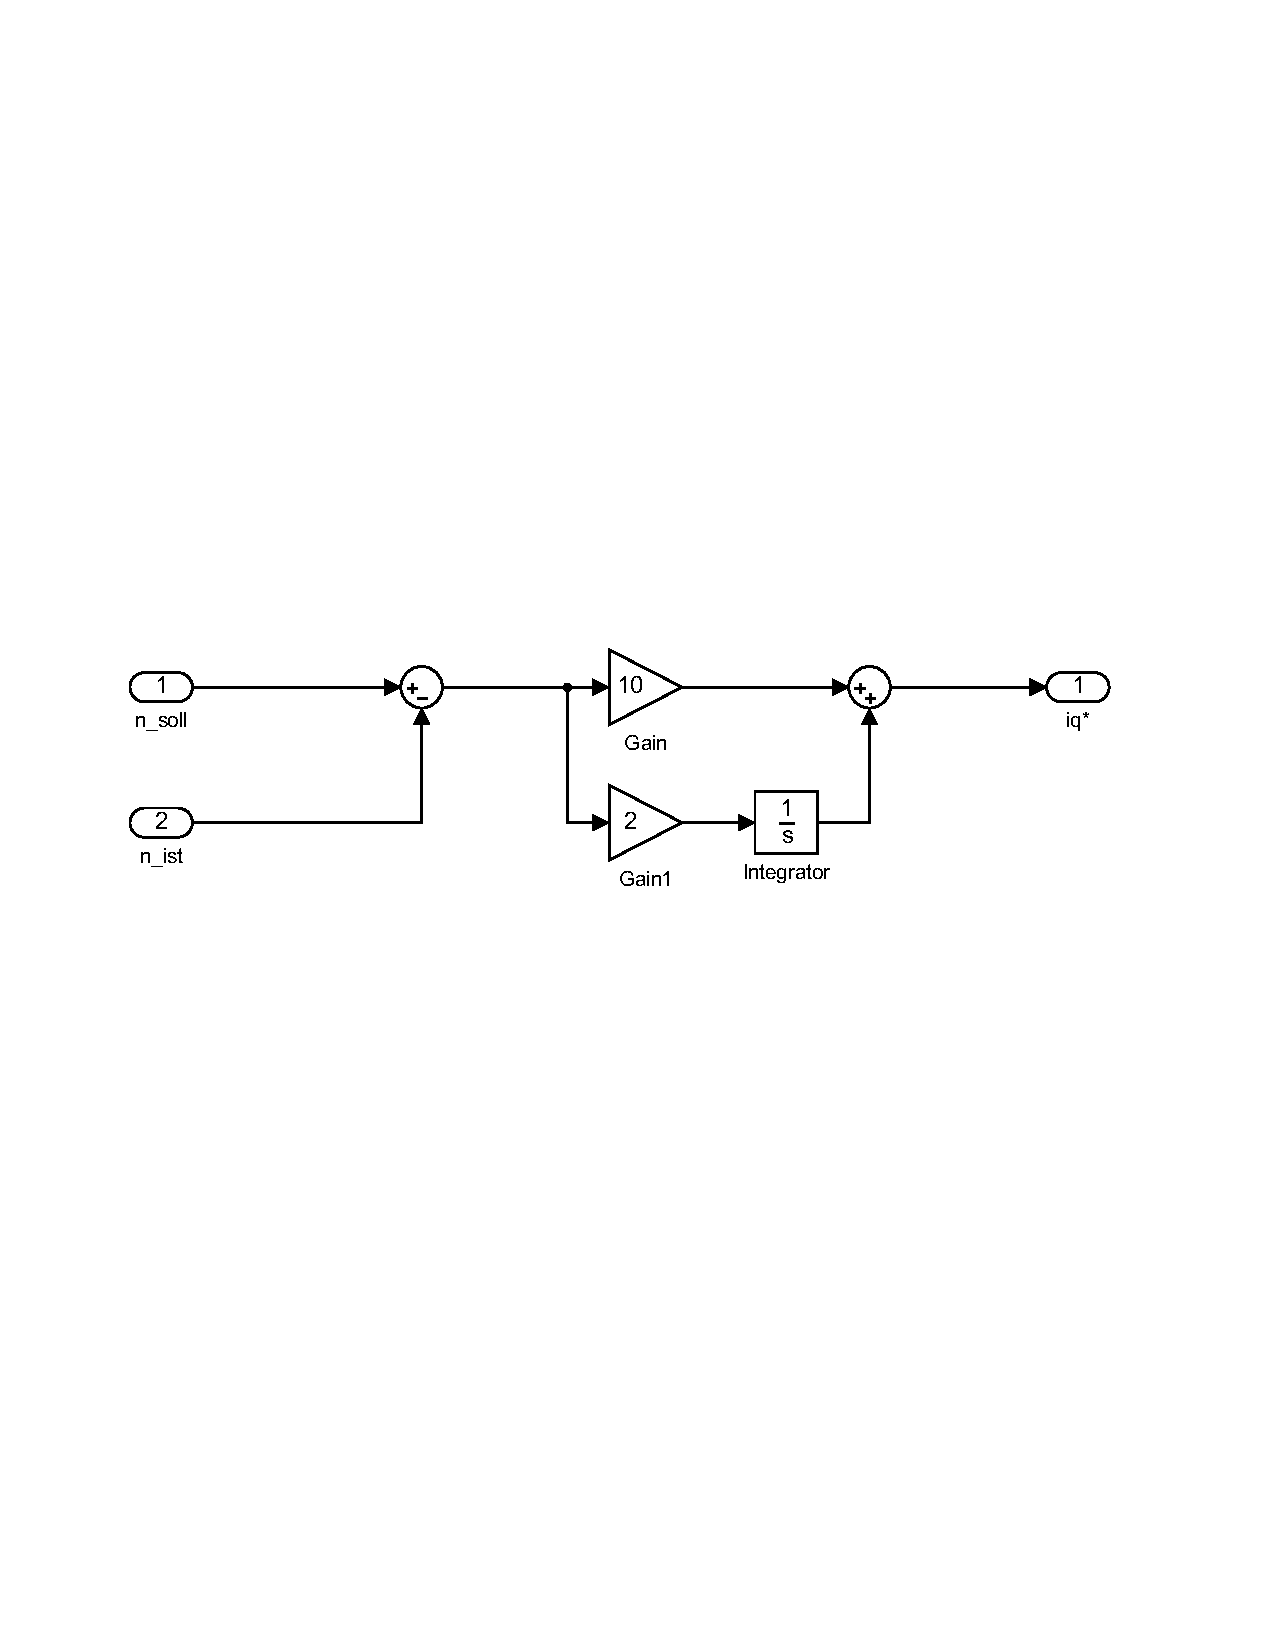
\includegraphics[width=\textwidth]{/simulink/drehzahl.pdf}
	\label{fig:drehzahl}
	\caption{Aufbau der Drehzahlregelung}
\end{figure}

Der Stromregler wird in Abbildung \ref{fig:stromregelung} gezeigt:

\begin{figure}[h]
	\centering
	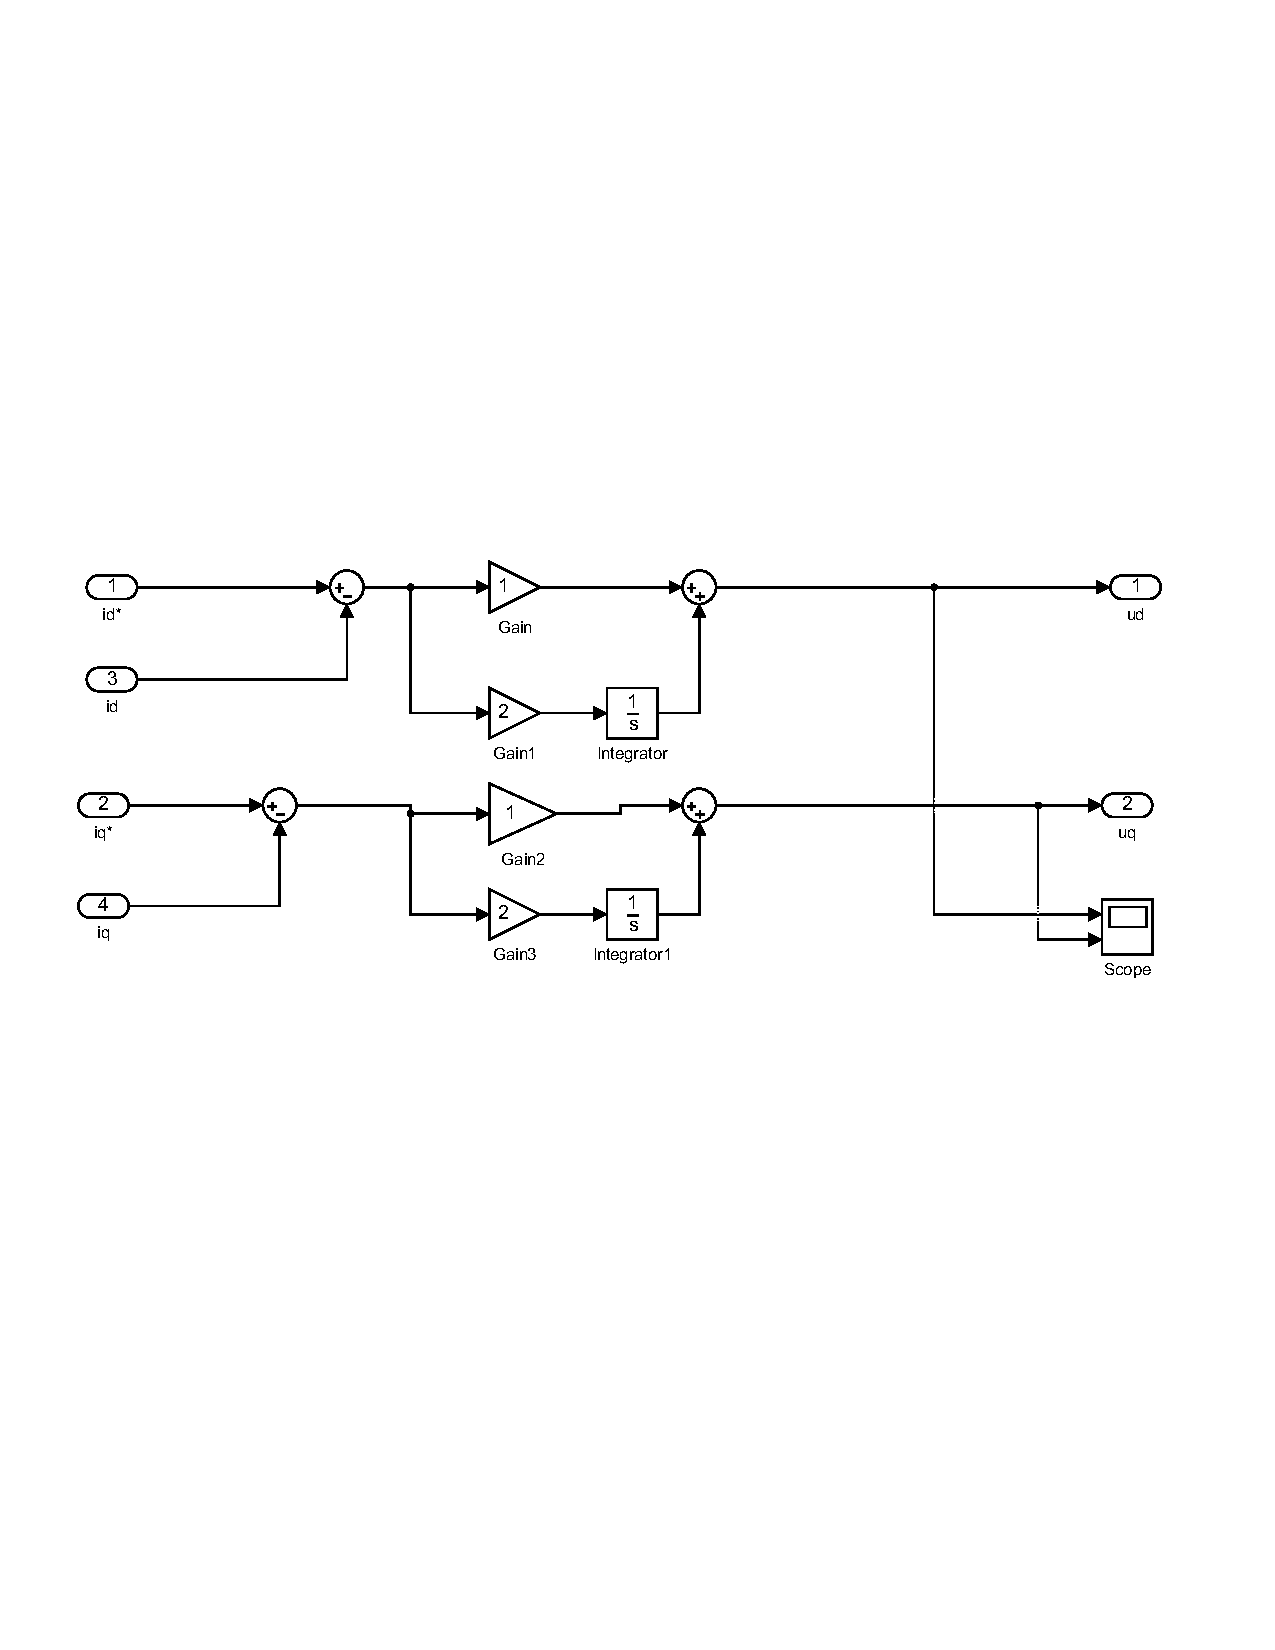
\includegraphics[width=\textwidth]{/simulink/stromregelung.pdf}
	\label{fig:stromregelung}
	\caption{Aufbau der Stromregelung}
\end{figure}

%%% Local Variables: 
%%% mode: latex
%%% TeX-master: "main"
%%% TeX-open-quote: "\\enquote{"
%%% TeX-close-quote: "}"
%%% LaTeX-csquotes-open-quote: "\\enquote{"
%%% LaTeX-csquotes-close-quote: "}"
%%% End: 
